\section{Baking in the tropics}

Depending on the temperature your fermentation speed adapts.
In a warmer environment everything is faster. In a colder
environment everything is slower.

This includes the speed at which your sourdough ferments
the dough but also the speed of enzymatic reactions. The
amylase and protease enzymes work faster, making more
sugars available and degrading the gluten proteins.

At around 22°C in my kitchen my bulk fermentation is ready
after around 10 hours. I am using around 20 percent of sourdough
starter based on the flour. In summer times the temperatures
in my kitchen sometimes increase to 25°C. In that case
I am reducing the sourdough starter to around 10 percent.
If I wouldn't do that my fermentation would be done after
around 4-7 hours. The problem is that the dough is quite
unstable when fermenting at this high speed. This means
that you are easily running into issues of overfermentation.
Finding the perfect sweet spot between fermenting enough
and not too much is becoming much harder. Normally you might
have a time window of 1 hour. But at the rapid speed it
might be reduced to a time window of 20 minutes. Now at
30°C ambient temperature things are way faster. Your bulk
fermentation might be complete in 2-4 hours when using
10-20 percent starter. Proofing your dough in the fridge
becomes almost impossible. As your dough cools down in the
fridge the fermentation also slows down. However cooling the
dough down from 30°C to 4-6°C in your fridge takes much
longer. Your dough is much more active compared to a dough
that starts at a temperature of 20-25°C. You might
end up overproofing your dough if you leave it overnight
in the fridge.

That's why I recommend that you reduce the amount of starter
that you use in the tropics to something at around 1-5 percent
based on the flour. This will slow down the fermentation
process significantly and provides you a bigger window
of time. Try to aim for an overall bulk fermentation of at
least 8-10 hours. Reduce the amount of starter to get there.

When making a dough try to use the same water temperature
as your ambient temperature. Assuming that the temperature
will climb to 30°C, try to start your dough directly
with 30°C water. This means that you can carefully rely on
a small fermentation probe that visualizes your fermentation
progress. The probe only works reliably if your dough temperature
is equal to your ambient temperature. Else the sample heats
up or cools down faster. So tread carefully when using
the sample in this case. It's always better to stop
the fermentation a little too early rather than too late.
Stretch and folds during the bulk fermentation
will help you to develop a better look and feel for
the dough. An expensive but possibly useful tool
could be a pH meter that allows you to perfectly
measure how much acidity has been created by the
lactic and acetic acid bacteria. In this case measure
the pH repeatedly and figure out a value that works
for your sourdough. In my case I tend to end bulk
fermentation at a pH of around 4.1. Please don't just
follow my pH value, it's very individual. Keep measuring
with different doughs to find out a value that works for you.

\section{My bread stays flat}
\label{sec:flat-bread-crumb}

A flat bread is in most cases related to your gluten
network breaking down fully. This is not bad, this
means you are eating a fully fermented food. However
from a taste and consistency perspective it might be
that your bread tastes too sour, or is not fluffy anymore.
Please also note that you can only make bread with
great oven spring when making wheat based doughs. When
starting with this hobby I always wondered why my rye
breads would turn out so flat. Rye has gluten yes, but
small particles called {\it hemicelluloses} (arabinoxylan and beta-glucan) \cite{rye-defects}.
prevent the dough from developing a gluten network like you can
do with wheat. Your efforts are in vain, your dough will
stay flat. Only spelt and wheat based doughs have the capability
to retain the CO2 created by the fermentation.

In most cases something is probably off with your
sourdough starter. This very often happens when the starter
is still relatively young and hasn't yet matured
at fermenting flour. Over time your sourdough
starter is going to become better and better at fermenting
flour. Keep your sourdough starter at room temperature
and then apply daily feedings with a 1:5:5 ratio.
This would be 1 part old starter, 5 parts flour,
5 parts water. This allows you to achieve a better
balance of yeast and bacteria in your sourdough.
Even better could be the use of a stiff sourdough
starter. The stiff sourdough starter boosts
the yeast part of your starter. This allows you
to have less bacterial fermentation, resulting
in a stronger gluten network towards the end
of the fermentation \cite{stiff+starter}. Please
also refer to the section ~\ref{sec:flat-bread-crumb} where
I explained more about overfermented doughs.

\begin{figure}[!htb]
  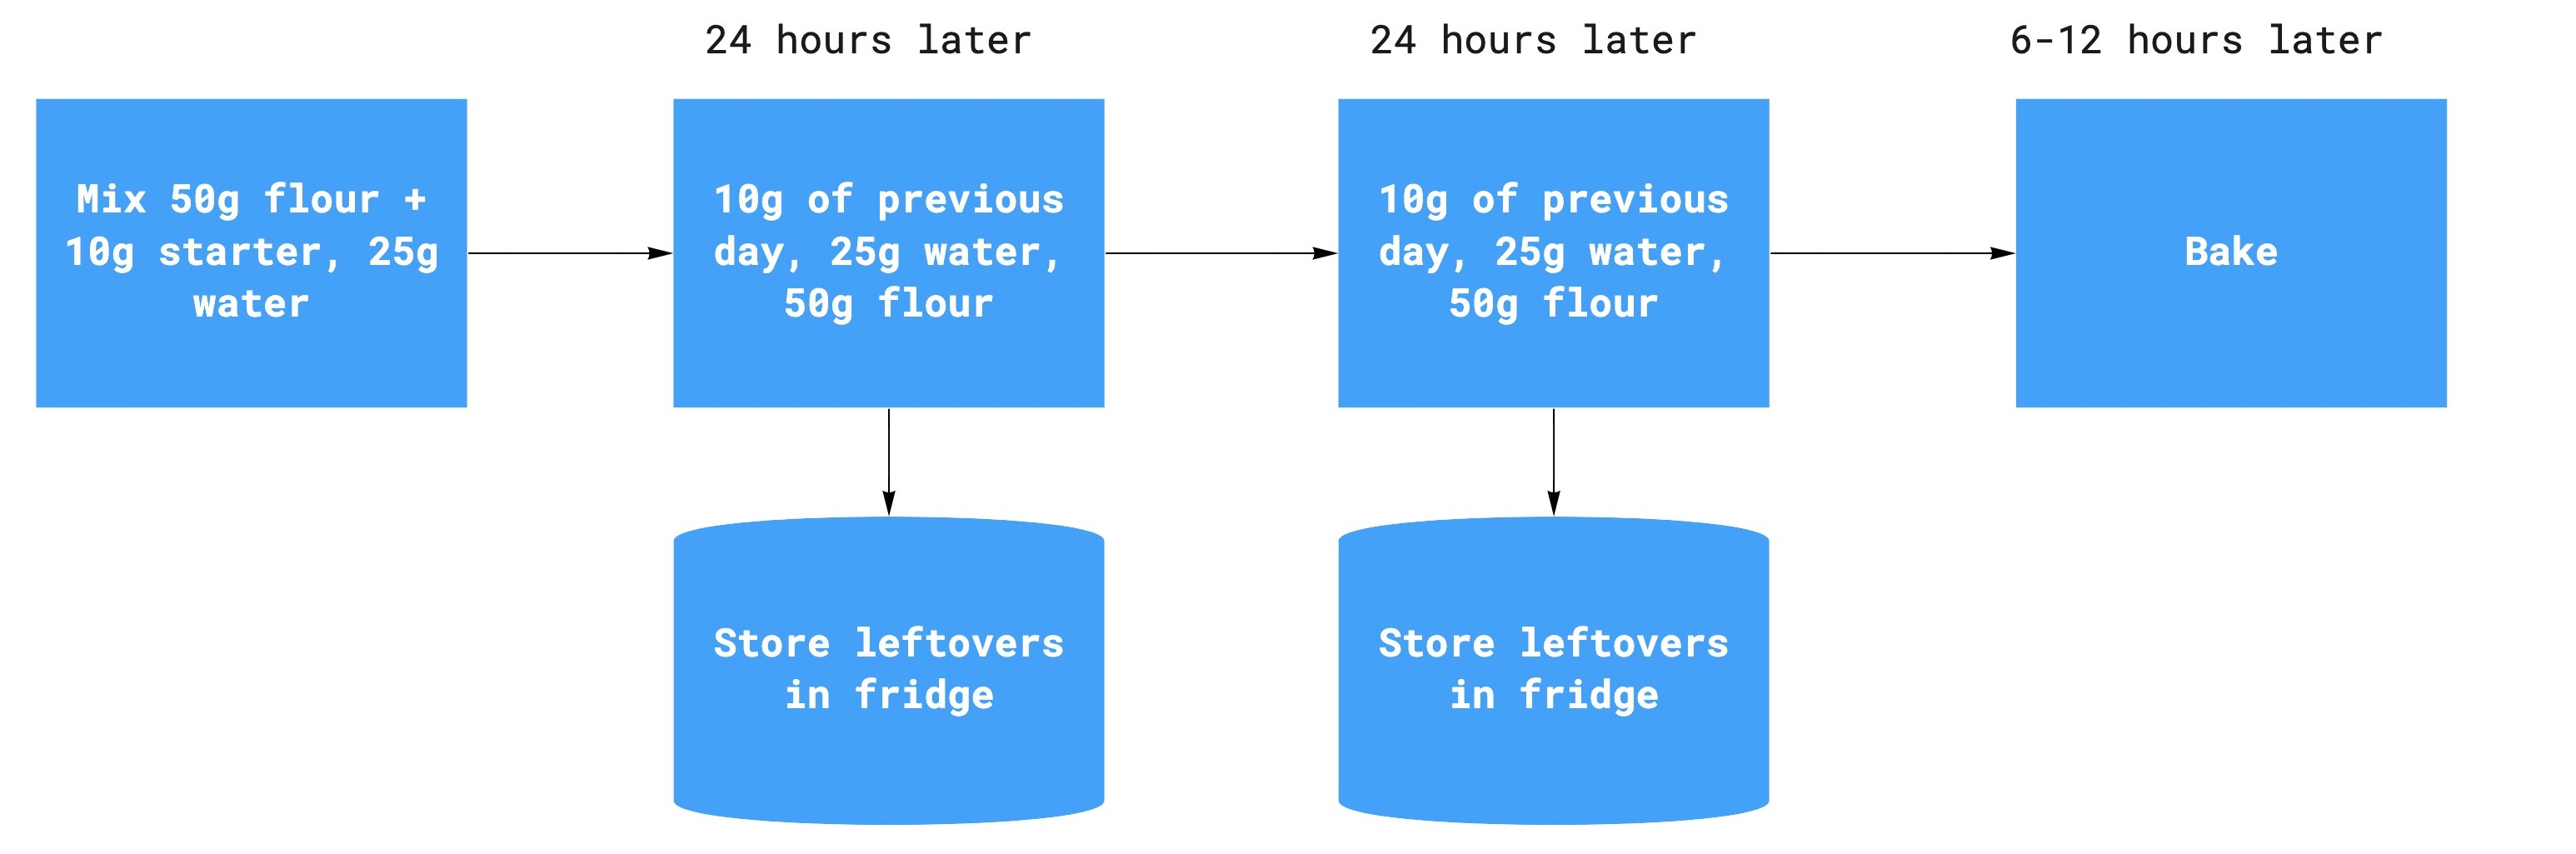
\includegraphics[width=\textwidth]{stiff-starter-conversion}
  \caption{The process to convert your starter into a stiff starter.}
  \label{fig:stiff-starter-conversion}
\end{figure}

Furthermore a stronger flour containing more gluten
will help you to push the fermentation further. This
is because your flour contains more gluten and will
take longer to be broken down by your bacteria. Ultimately
if fermented for too long your dough is also going
to be broken down and will become sticky and flat.

To debug whether the excess bacterial fermentation is the issue,
simply taste your dough. Does it taste very sour? If yes,
that's a good indicator. When working the dough, does it
suddenly become very sticky after a few hours? That's a
another good indicator. Please also use your nose to note
the smell of the dough. It shouldn't be too pungent.

\section{I want more tang in my bread}

To achieve more tang in your sourdough bread you have
to ferment your dough for a longer period of time.
Over time the bacteria will metabolize most of the
ethanol created by the yeast in your dough. The bacteria
mostly produces lactic and acetic acid. Lactic acid
is chemically more sour than acetic acid but sometimes
not achieved as sour. In most cases a longer fermentation
is what you want. You will either need to utilize a loaf
pan to make your dough or use a flour that can withstand
a long fermentation period. A flour like this is typically
called a {\it strong flour}. Stronger flours tend
to be from wheat varieties that have be grown in more
sunny conditions. Because of that stronger flours tend
to be more expensive. For freestanding loaves I recommend
to use a flour that contains at least 12 percent protein.
Generally the more protein the longer you can ferment your dough.

Another option to achieve a more sour flavor could be to
use a starter that produces more acetic acid. Acetic acid
bacteria tend to be more common in rye starters (source needed).
Chemically the acetic acid isn't as sour, but when tasting
it will seem more sour. Make sure to use a starter that is at
a hydration of around 100 percent. Acetic acid production
requires oxygen. A too liquid starter tends to favor lactic
acid production because the flour is submerged in water, no
oxygen can reach the fermentation after a while.

\begin{figure}[!htb]
  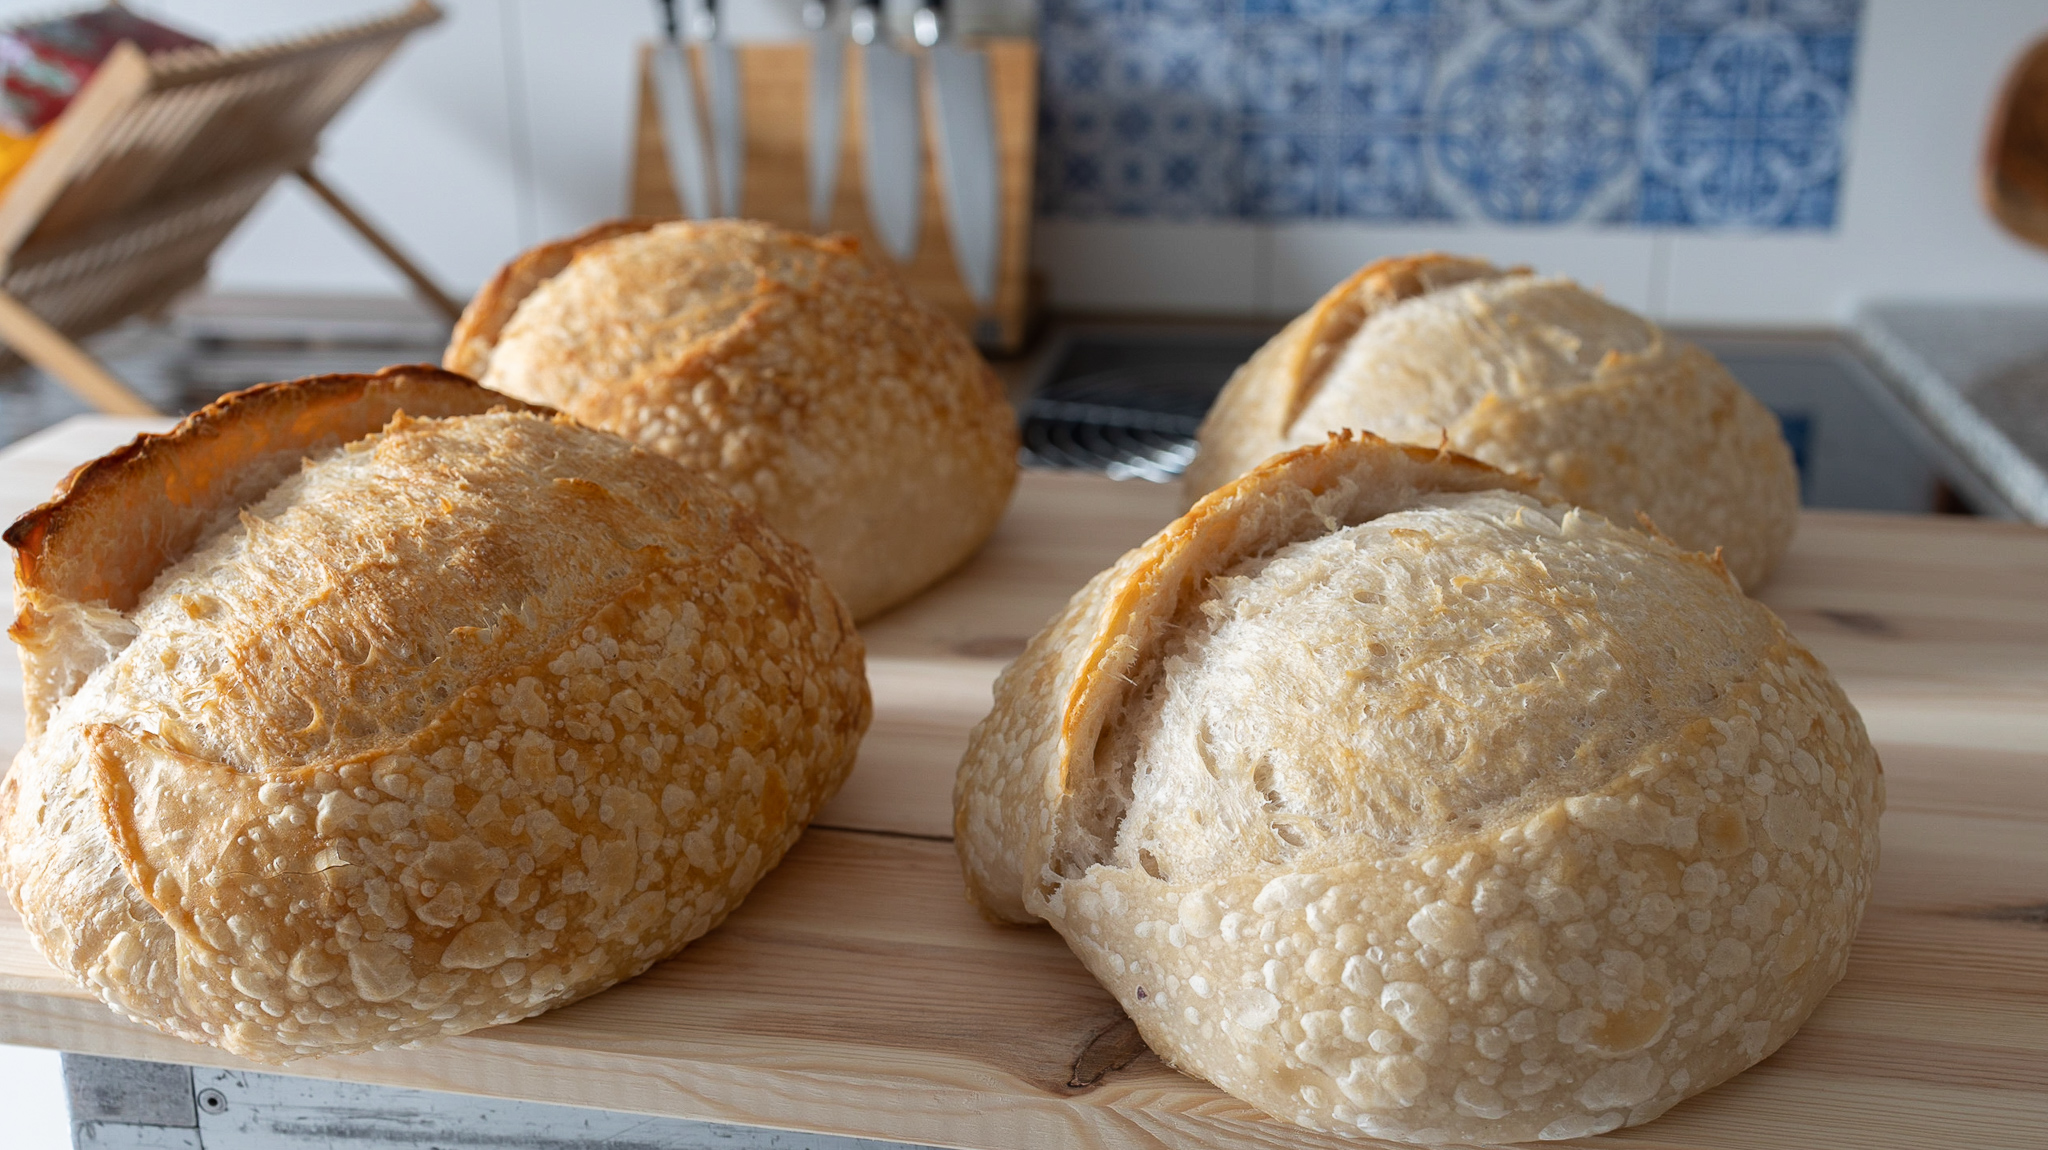
\includegraphics[width=\textwidth]{parbaked-bread.jpg}
  \caption{A half-baked bread, known as "parbaked".}
  \label{fig:parbaked-bread}
\end{figure}

Another more easier option could be to bake your sourdough
twice. I have observed this when shipping bread for my micro
bakery. The idea was to bake my bread for around 30 minutes
until it's sterilized, let it cool down and then ship it
to customers. Once you receive it you just bake it again
for another 20-30 minutes to achieve the desired crust and
then you can eat it. Some of the customers reported a very sour
tasting bread. After investigating a bit more it became
crystal clear. By baking the bread twice you don't boil
as much of the acid during the baking process. Water
evaporates at around 100°C while acetic acid boils at
118°C and lactic acid at 122°c. After baking for 30 minutes
at around 230°C some of the water has started to evaporate,
but not all the acid yet. If you were to continue to bake more
and more of the acid would start to evaporate. Now if you were
to stop baking after 30 minutes, you would typically have reached
a core temperature of around 95°C. Your dough would need
to be cooled down again to room temperature. The crust would
still be quite pale. Then A couple of hours later you start
to bake your dough again. Your crust would become nice and
dark featuring delicious aroma. The aroma is coming from the
maillard reaction. However the core of your dough still won't
exceed the 118°C required to boil the acid. Overall your
bread will be more sour. The enhanced acidity also helps
to prevent pathogens from entering your bread. The bread
will be good for a longer period of time.

\section{My bread is too sour}
\section{Fixing a moldy sourdough starter}
\section{My bread flattens out after shaping}
\section{Liquid on top of my starter}
\section{Why does my starter smell like acetone}
\section{My crust becomes chewy}